\begin{onehalfspacing}
\chapter{Methodology and Implementation}
\section{Process Description}
Process is a program currently in execution. It is also a basic unit of execution for an Operating System (OS). Process includes wither a user process or its own system/kernel process or an idle process if it has nothing else to do. To run a process OS needs to allocate some physical memory for it and load the address of first instruction to execute in Central Processing Unit (CPU). Every process has a virtual memory address space containing a range of digits depending on the architecture of the system, and the number of bits available to store addresses in registers. These virtual addresses requested by the CPU are than converted into actual physical addresses during runtime. After the process gets executed, its removed from the memory to free up the space. Each process is identified by some id's mainly called as pid so as to reference processes. 

\section{Process States}
Process state is the condition of process at particular instance of time during execution. It also defines the current position and status of a process which gives detail of process at that particular instant whether it is executing or not. Some of the states of process are:
\begin{enumerate}

    \item \textbf{New}
    \par Process is created when a program is called from secondary memory to primary memory. In this phase,process is about to be created.
    
    \item  \textbf{Ready}
    \par After the process is created, it enters into ready state where it gets ready to run. The process gets loaded into primary memory ready for execution. The ready to run process gets time taken for execution from CPU. A ready queue is maintained so as to process ready processes.
    
    \item  \textbf{Waiting}
    \par The process enters into waiting state when the current process is kept into hold and other process are allowed for execution. This happens when process tries to access resource that is already acquired by other process and it has to wait until a lock is released by other process.
    
    \item  \textbf{Executing}
    \par When CPU chooses process to execute, it inters into run state. Here all the instructions are executed by any one of the available CPU cores.
    
    \item  \textbf{Suspended}
    \par It denotes that process was initially in ready state that got swapped out from main memory and placed into secondary memory. Once the process is demanded by CPU, it is again brought into main memory.
    
    \item  \textbf{Terminated}
    \par Process once fully executed releases all the resources and gets terminated. The resource includes previously when it was allocated into main memory

\end{enumerate}

\newpage
\begin{figure}[h]
    \centering
    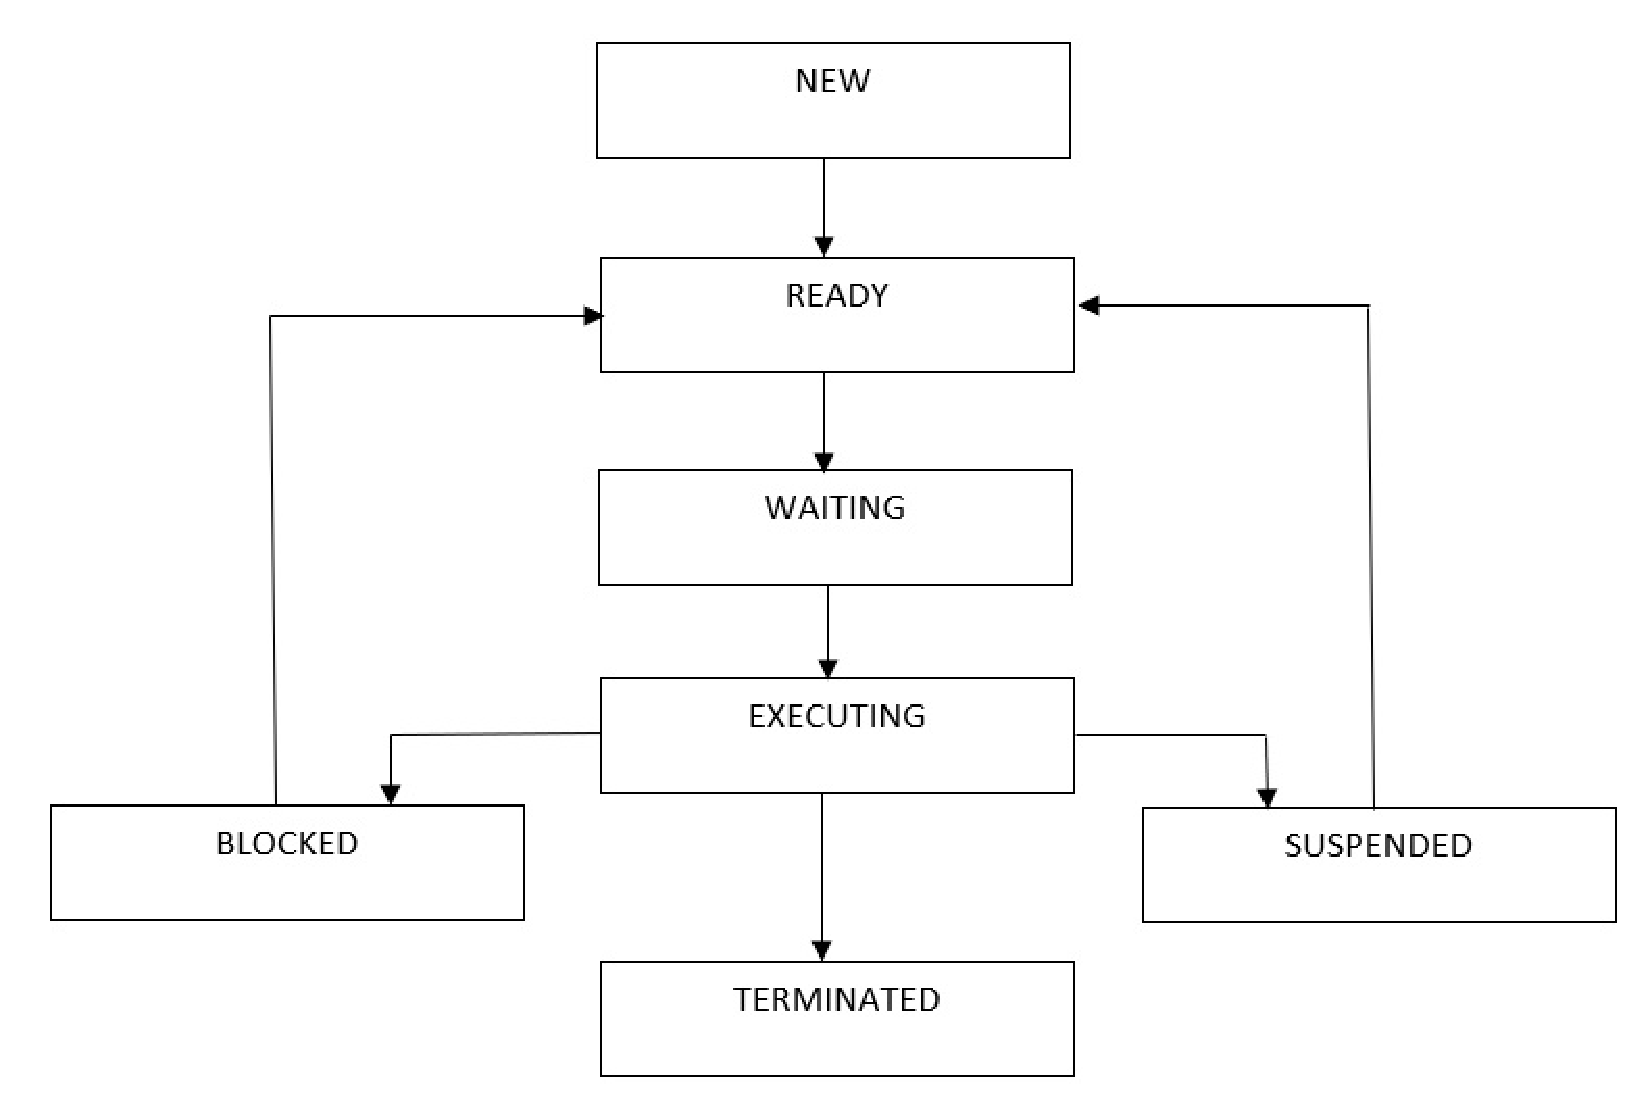
\includegraphics[width=15cm]{./process_state.eps}
    \caption{Process State}
    \label{fig:my_label}
\end{figure}

\section{Process Creation}
In Operating System once a request is made to execute a program, it gets converted into process. Programs Operating system identifies process by assigning it a unique process identifier (PID) and inserts that particular process into process table. Newly created process is allocated all the required resources such as memory space, space for its Process Control Block(PCB) etc. Created process is kept in a ready queue for execution and maintained by a scheduler so as to make each and every process run without any interruption. 
\newpage
\section{Process Queue}
For each of the process states, various types of queues are maintained. For each state, PCB to the process is also stored in the queue so as to process according to PCB information. Once the process moves from one state to another state, PCB is also unlinked from previous state and added to the new state queue. Queue is highly maintained for each states so as to execute all the processes smoothly. Queue also maintains the sequence of processes that are waiting to be executed.
\begin{figure}[h]
    \centering
    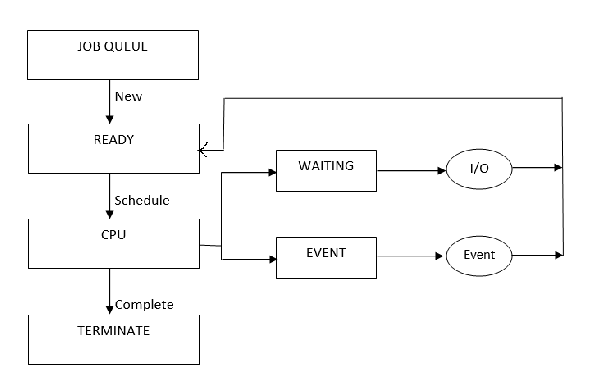
\includegraphics[width=15cm]{./proess_queue.eps}
    \caption{Process State}
    \label{fig:my_label}
\end{figure}


















































 


\end{onehalfspacing}